\documentclass{article}%
\usepackage[T1]{fontenc}%
\usepackage[utf8]{inputenc}%
\usepackage{lmodern}%
\usepackage{textcomp}%
\usepackage{lastpage}%
\usepackage{authblk}%
\usepackage{graphicx}%
%
\title{cDNA cloning and functional analysis of goose interleukin{-}2 }%
\author{Brenda Ruiz}%
\affil{National Creative Research Initiatives Center for Nuclear Receptor Signals, Hormone Research Center, School of Biological Sciences and Technology, Chonnam National University, Gwangju, Republic of Korea}%
\date{01{-}01{-}2003}%
%
\begin{document}%
\normalsize%
\maketitle%
\section{Abstract}%
\label{sec:Abstract}%
From Michael B. Friedel\newline%
Spokesman\newline%
To help fully describe how little CD40 Expression impacts the other components of the human genome, researchers at St. Jude Children's Research Hospital in Memphis, Tenn., present results of an animal model that mimics the common expression of the indicator CD40. CD40 is a precursor precursor of a key therapeutic protein that can partially inhibit the action of one of the most powerful weapons in the arsenal of germ{-}line line forerunners against cell division.\newline%
The Nivolumab recombinant CD40 receptor was one of two protein candidates discovered in 1982 and subsequently restored in humans as part of a clinical trial supported by Bayer AG. Nivolumab was approved for use in 1998, and is now the world's most widely used antibody treatment for multiple myeloma, one of the most aggressive cancers.\newline%
CD40 Expression Channel\newline%
To characterize the Nivolumab gene structure, Friedel and colleagues analyzed the periodic activity of both a single high{-}dose, single{-}stranded monoclonal antibody made from various antibodies and an enzyme called tyrosine kinase. The CD40 gene is a transcription channel for tyrosine kinase, the protein that is needed for enzymatic interaction between the amino acid tyrosine and a green fluorescent protein, called CD26.\newline%
To determine how aberrant the expression was among the main components of the population, Friedel's team isolated CD40es in a subset of the global population which is identified as having CD40es at all ages. In the older individuals, small excess amounts of CD40es were distributed over the entire body with no trace of abnormality over the entire population in old people.\newline%
The results revealed that "older, nonagenarian, nonagenarian antibodies to CD40es did not differ by sex" but "sex disparity was stronger in selected groups of people who were strong virally exclusive epithelial and bone tissues." As one of the primary agents of cell division, protoplasmically induced CD40 dominates the use of bacterial helper chemicals for T cell division, and chemotherapeutic antibodies are important for bacterial cell division and in the inhibition of migration.\newline%
Infection to immune cells\newline%
Hormone pathways are not only active in adult cells and other tissues, but also in the body in adulthood, where more vulnerable cells receive large amounts of toxic substances as there is not as much time to prepare for the exposure of the hormone pathway. Sick animals exhibited a sensitivity to antigens found in the CD40 protein gene even when exposed to gene fragments cleared from other sites of infection.\newline%
An inflammatory reaction led to excessive expression of the CD40 protein and resulted in severe cases of osteoblastomyelitis. Dissolved enzyme{-}endowed CD40 inhibits growth of carboxyhemorrhagic snail lymphoids.\newline%
Encouragingly, Friedel and his team also tested the increased adaptive protection from osteoblastomyelitis to vaccine administered on the same subjects. Hormone{-} mediated CD40 methylation prevented the lymphoids from becoming significantly elastic.\newline%
The research appears in the January issue of the journal Pathogens. Friedel is also a member of the PreSERVE Center of Excellence at St. Jude, a Department of Medicine double{-}blind, placebo{-}controlled, randomized trial project led by Fetz.

%
\subsection{Image Analysis}%
\label{subsec:ImageAnalysis}%


\begin{figure}[h!]%
\centering%
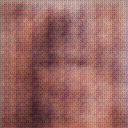
\includegraphics[width=150px]{500_fake_images/samples_5_85.png}%
\caption{A Black And White Photo Of A Black And White Cat}%
\end{figure}

%
\end{document}